\chapter{Analysis techniques}
\section{Strategy for searching for four top quarks \label{sec:Strategy}}

The LHC has been said to be a ``top factory'' due to the large cross sections for \ttbar production at 8 TeV and 13 TeV, \fxnote*{ref}{253~pb and 831~pb} respectively. Hence most analyses within the CMS collaboration which work on top quark physics study \ttbar production. In the SM, each of the top quarks will decay to a W boson and a b quark almost 100$\%$ of the time. The final state of the \ttbar process in the detector is defined by whether the W boson decays leptonically into a lepton and neutrino or hadronically into two quark jets. The standard strategy is to require two b-jets to be present in the event and 0, 1 or 2 leptons depending on the final state defined as \emph{all-hadronic}, \emph{semi-leptonic} and \emph{dileptonic} respectively where 6, 4 or 2 total number of jets are required. 

\begin{figure}[ht!]
\centering
    \includegraphics[width=0.7\textwidth]{images/Analysis/Ttbar_decay_channels.png}
    \caption{The possible decay channels for \ttbar production where the area of each final state is proportional to its branching ratio.}
    \label{fig:ttbarDecay}
\end{figure}
%picture from wiki By Nazar Bartosik - http://bartosik.pp.ua/hep_sketches/tt_decay_channels, CC BY 4.0, https://commons.wikimedia.org/w/index.php?curid=49739344

Not all \ttbar events will be captured within the selection due to inefficiences in tagging b-jets, identifying leptons and reconstructing jets. As the rate of \ttbar production is so high at the LHC, this selection still provides a large enough sample of events to have statistically significant studies.\\

The strategy for selecting \tttt events while suppressing background processes is similar to the \ttbar selection but with the requirement of additional two jets. The small cross section for \tttt production in the SM, \fxnote*{ref}{1.3~fb at 8~TeV and 9.2~fb at 13~TeV} dictates the selection. It would be preferential to require 4 b-jets in the selection to obtain the highest signal to background ratio, however this would have a detrimental effect on the overall amount of \tttt found in the selection due to some b-jets not being identified correctly or being within the acceptance of the detector. Similarly, it is not possible to require a jet per quark hadronising in the detector in a \tttt final state as some of the jets may be merged or may not be within the acceptance of the detector. However, it will be discussed in section~\ref{sec:Cats} how a looser selection can be used to an advantage to constrain the main background process.

This thesis will focus on the single lepton channel where only single muon and single electron final states are considered. As can be seen from~\ref{fig:ttttDecay}, the single lepton channel represents the largest branching ratio of the four top quark decay channels. The dilepton channel, which has the second largest branching ratio will also briefly be discussed in chapter~\ref{c:Run2} as it was combined with the single lepton channel to achieve an increased sensitivity on the analysis. In the dilepton channel also only final states with muons and electrons were considered. The criteria which each channel are required to pass are called the \emph{Baseline Event Selection}.

\begin{figure}[ht!]
\centering
    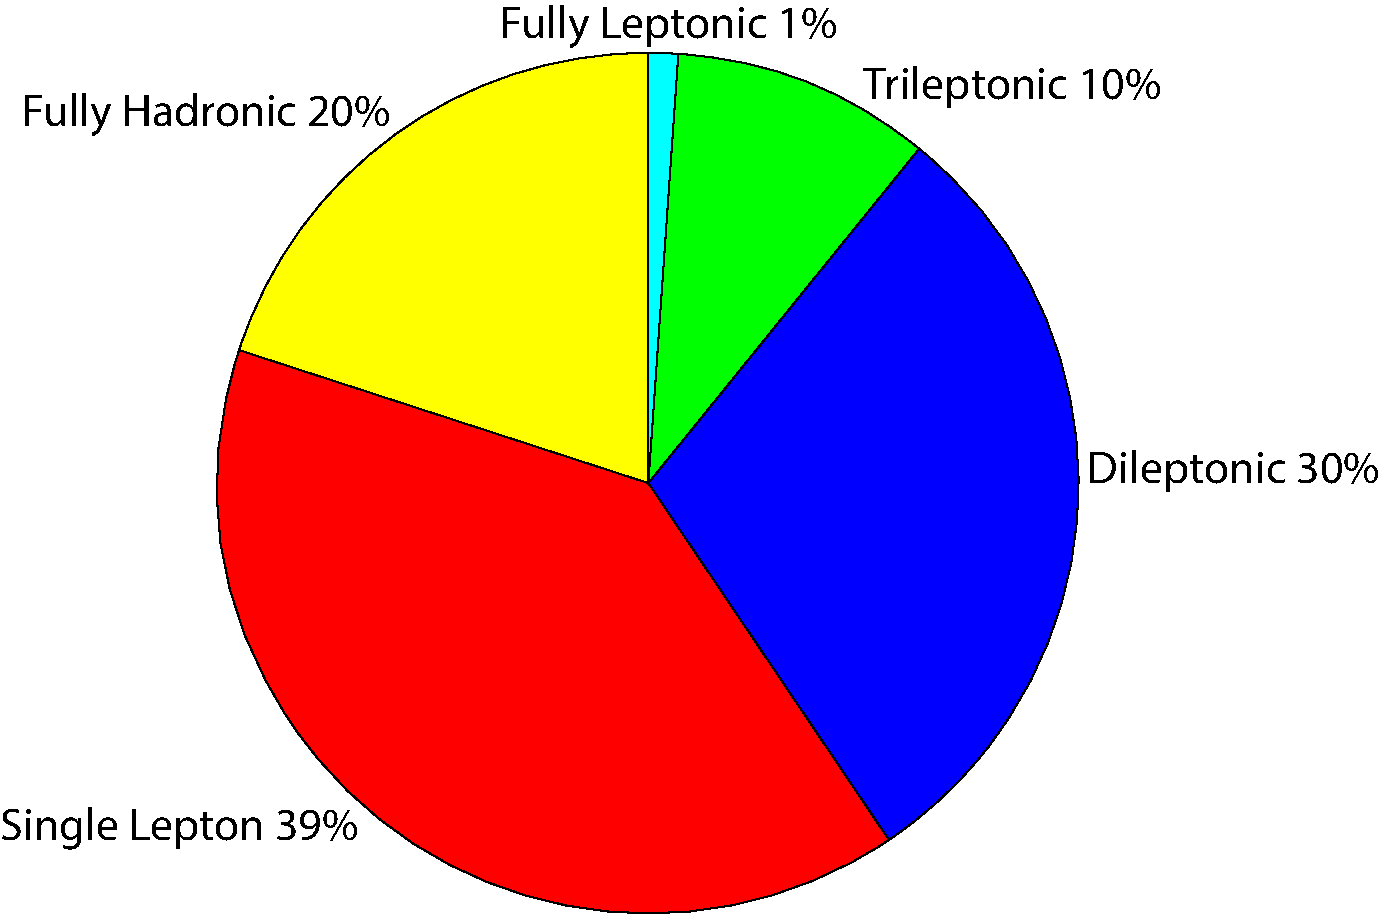
\includegraphics[width=0.5\textwidth]{images/Analysis/FourTopBR.pdf}
    \caption{The possible decay channels for \tttt production}
    \label{fig:ttttDecay}
\end{figure}

\section{Signal and background processes}
\label{sec:sigback}
\fxnote{Discuss four top signal process and what that would look like in the detector}
\fxnote{Discuss background process which could mimic 4tops}
\fxnote{Add feynman diagram}


\section{Corrections to the simulation}
\label{sec:Calibrations}
Many of the parameters which go into simulating each particle physics process are not precisely known. therefore they are tuned to produce the simulation which best matches the data observed. This simulation will still have residual discrepancies from data which can be measured and accounted for by producing \emph{scale factors} (SF) which are usually \pt and $\eta$ dependent and may be dependent on other factors such as jet flavour. These SFs are used to produce a per-event weight for simulated events such that the overall distributions more closely match data. 


\subsection{Pileup modelling}
\label{sec:pile-up}
The distribution of the number of primary vertices varies between data and simulation for a given luminosity. This can be taken into account by looking at the number of events for each number of primary vertices in data and simulation and applying the scale factor, $SF_{PU}\left( i \right)$ to simulation, where \emph{i} is the number of vertices.

\begin{equation}
SF_{PU}\left( i \right) = \frac{N_{events}^{Data}}{  N_{events}^{sim}} 
\label{eqn:PUSF}
\end{equation}

$SF_{PU}$ is derived using \emph{minimum bias} data and simulation. This means that the data have been collected using a much looser trigger than those used to detect interesting physics events. 

\subsection{b tag modelling ~\label{sec:btagModelling}}

\subsubsection{Method 1 ~\label{subsec:method1btag}}
There are residual differences between b tagging efficiencies measured by CMS in data and the efficiencies as measured in simulation as it is difficult to simulate the fragmentation and hadronisation of b-quarks. 
The b-tagging efficiencies are measured for each of the CSVL, CSVM, and CSVT working points in bins of \pt and $\eta$. Depending on which working point was used in an analysis a scale factor, $SF(\eta, P_{T})_{i}$,  can be applied to the simulation for each jet. This is dependent on the \pt, $\eta$ and flavour, \emph{i}, of the jet, shown in equation~\ref{eqn:sfbtagnorm}, where $\epsilon(\eta , \pt)^{data}_{i}$ is the efficiency for a jet to be tagged as a b-jet in data and $\epsilon(\eta , \pt)^{sim}_{i}$ is the efficiency for identifying a jet as a b-jet in simulation.

\begin{centering}
\begin{equation}
SF(\eta, P_{T})_{i} = \frac{\epsilon(\eta , \pt)^{data}_{i}}{\epsilon(\eta , \pt)^{sim}_{i}}
\label{eqn:sfbtagnorm}
\end{equation}
\end{centering}
Separate scale factors are defined for b and light (u, d, s, g) jets. Scale factors for c jets are taken to be the same as for b jets. A weight, $\omega_{btag}$ can be applied to simulated events. The method proceeds by defining the probability of an event in simulation producing a given number of tagged and untagged jets, \emph{P(MC)},:

\begin{centering}
\begin{equation}
P(MC) = \prod_{tagged jets}\epsilon^{sim}_{i} \times \prod_{untagged jets}(1- \epsilon^{sim}_{i})
\end{equation}
\end{centering}
where $\epsilon_{i}$ is the efficiency of tagging a jet of flavour $i$ with the CSV criterion in simulation. While the probability of an event in data producing a given number of tagged and untagged jets, P(DATA), is defined as follows:


\begin{centering}
\begin{equation}
P(DATA) = \prod_{tagged jets}SF_{i}\cdot\epsilon^{sim}_{i} \times \prod_{untagged jets}(1- SF_{i}\cdot\epsilon^{sim}_{i})
\end{equation}
\end{centering}
where SF is the appropriate scale factor for a jet of flavour $i$. 

An overall weight to be applied to each event depending on the jet content can be derived from these scale factors using Eqn.~\ref{eqn:weightbtagnorm}. This weight, $\omega_{btag}$, must be applied to the selected simulation events in order to predict the correct event yield in data.

\begin{centering}
\begin{equation}
 \omega_{btag} = \frac{P(DATA)}{P(MC)}
 \label{eqn:weightbtagnorm}
\end{equation}
\end{centering}

\subsubsection{Method 2 ~\label{subsec:method2btag}}

Alternatively, the measurements at each working point can be used to fit the shape of the CSV distribution and provide scale factors in bins of \pt and $\eta$ for each jet flavour. Therefore the scale factors for each jet can be derived from the \pt and $\eta$, CSV discriminator value and for each jet flavour as seen in equation~\ref{eqn:btagcsv}. For this method, the jet flavours are defined as heavy for bottom quarks and light for u, s, d, g whilst c-quarks are given $\textrm{SF} = 1$. Further details of the CSV reshaping can be found in Ref.~\cite{CMS-NOTE-2013-130}.

\begin{equation}
% \textrm{SFjet}_{\textrm{B}} \left(\textrm{CSV},\pt,\eta \right) = \frac{\textrm{Data} - \textrm{MC}_{\textrm{A}}}{\textrm{MC}_{\textrm{B}}} ~~;~~ \textrm{A, B = heavy flavour, light flavour or vice versa}
\textrm{SFjet}_{\textrm{i}} \left(\textrm{CSV},\pt,\eta \right) = \frac{\njets^{Data} - {\njets^{MC}}_{,j}}{{\njets^{MC}}_{,i}} ~~;~~ \textrm{i, j = heavy flavour, light flavour or vice versa}\label{eqn:btagcsv}
\end{equation}

An event weight can be derived by taking the product of the per-jet scale factors as seen in equation~\ref{eqn:btagcsvtot}.

\begin{equation}
\textrm{SF}_{\textrm{total}} = \prod_{i}^{\njets}\textrm{SFjet}_{i}
\label{eqn:btagcsvtot}
\end{equation}

\subsection{Heavy flavour jet modelling ~\label{ttbbmod}}
% There is a discrepancy between data and simulation in the distribution of the number of b-tagged jets (\nbtags) at higher numbers of b-tags which suggests that the amount of heavy flavour jets in \ttbar events is incorrectly simulated.
The extra jets in \ttbar events can come from processes such as gluon splitting pair-producing \bbbar. These \ttbb events are most likely to resemble the features of the \tttt signal events and so it is essential that the proportion of them in simulation is correctly modelled. Table~\ref{tab:heavyflavR} shows the heavy flavour ratio $R=\heavyflavourone~/~\heavyflavourtwo$ as measured by CMS at 8~TeV and 13~TeV in data and in simulation. To incorporate this ratio into the analysis, the MC truth information of the \ttbar$+$jets (MC) sample is used to split the sample into \ttbb, \ttcc and \ttll, where l denotes light quarks and gluons (\cPqu, \cPqd, \cPqs, \cPg).  A scale factor SF = R(Data)~/~R(Sim) is derived from the information in table~\ref{tab:heavyflavR} which is applied to the \ttbb events. Another SF is applied to \ttll to preserve the total number of \ttbar events.


\begin{table}[htpb!]
\footnotesize
\begin{center}
\begin{tabular}{|l|l|l|l|}
\hline
$\sqrt{s}$ (TeV)                         & R(Data)  (\%)                                                                             & R(Sim) (\%)       & SF   \\
\hline
8~\cite{Khachatryan2015132}  & $2.2 \pm 0.4 \left( \textrm{stat.} \right) \pm 0.5 \left(\textrm{sys.} \right)$ & 1.6 $\pm$ 0.2 & 1.35 \\
13~\cite{CMS-PAS-TOP-16-010} & $2.2 \pm 0.3 \left( \textrm{stat.} \right) \pm 0.6 \left(\textrm{sys.} \right)$ & 1.2 $\pm$ 0.1 & 1.83 \\
\hline
\end{tabular}
\caption{Ratio of $R=\heavyflavourone~/~\heavyflavourtwo$ for Data and Simulation at 8 TeV and 13 TeV alongside the scale factor derived for R(Data)~/~R(Sim)}
\label{tab:heavyflavR}
\end{center}
\end{table}

\subsection{Lepton modelling}
A weight is applied to events which is dependent on the selected leptons $\eta$, $\pt$ and lepton flavour. The scale factors for each source of efficiency are designed to be multiplicative and the final event weight can be found in equation~\ref{eqn:leptonW}

\begin{equation}
\omega_{lepton} = SF_{iso}\times SF_{id}\times SF_{reco}\times SF_{trig}
\label{eqn:leptonW}
\end{equation}

\subsection{Top \pt modelling}

The top quarks which are reconstructed in \ttbar enriched regions of data tend to have a softer \pt spectrum than in \ttbar simulation. A scale factor can be derived as a function of the \pt of the top at generator level of the simulation (before it is reconstructed by the detector). The event weight can be derived by multiplying the independent SFs for each (anti-)top in the event and is shown in equation~\ref{eqn:topptW}. This SF is only applied to \ttbar simulation samples.

\begin{equation}
\omega_{topPt} = SF(\textrm{top}~\pt)\times (\textrm{anti-top}~\pt)
\label{eqn:topptW}
\end{equation}

\subsection{Jet multiplicity modelling \label{subsec:alphaS}}
Good modelling of the jet multiplicity distribution up to a large number of jets in the main \ttbar background is highly important for this analysis because as the number of jets increases, the signal to background ratio increases. Hence, the higher jet multiplicities have the highest sensitivity in separating the signal \tttt process and the background \ttbar process. It is essential that \ttbar is well modelled in this high jet multiplicity region. 
Particularly at 13 TeV the simulation was larger than data in the higher \njets bins. The value of $\alpha_S$ in the \ttbar Powheg+Pythia8 sample used in the analysis in chapter~\ref{c:Run2} is 0.137, however the best tune was observed to have a value of $\alpha_S=0.113^{+0.012}_{0.010}$. A scale factor was therefore calculated by CMS in order to improve the modelling of the \njets distribution. 

\section{Multi-jet background estimation}
\label{sec:QCDbackground}
The presence of multi-jet events within the signal region defined by the baseline selection is investigated in this section. \fxnote*{why?}{It is rare for multi-jet events to have a highly energetic undetectable particle}. Therefore, the $\MET$ distributions for multi-jet events typically peak at low values, not necessarily at zero as some jets may be outside of the acceptance of the detector or mis-measured. Due to the small number of events which pass the baseline event selection and the difficulty in simulating QCD events, it is not possible to use multi-jet simulation to estimate this background. In this case, a data-driven method known as the \fxnote*{ref?}{``ABCD method''} may be used. This method proceeds by selecting two uncorrelated variables from the object or baseline selection and defining three control regions (A,B,C) and one signal region, D, in the 2-dimensional phase space of these variables as shown in Fig.~\ref{fig:ABCDdiagram}. A selection is made in each variable which defines one quadrant of the phase space as the signal region.  The event variable \MET and the lepton variable RelIso were selected as they are \fxnote*{uncorrelated proof??}{uncorrelated} where the signal is defined in a low RelIso and higher \MET region.\\

\begin{figure}[ht!]
\begin{center}
\subfloat{
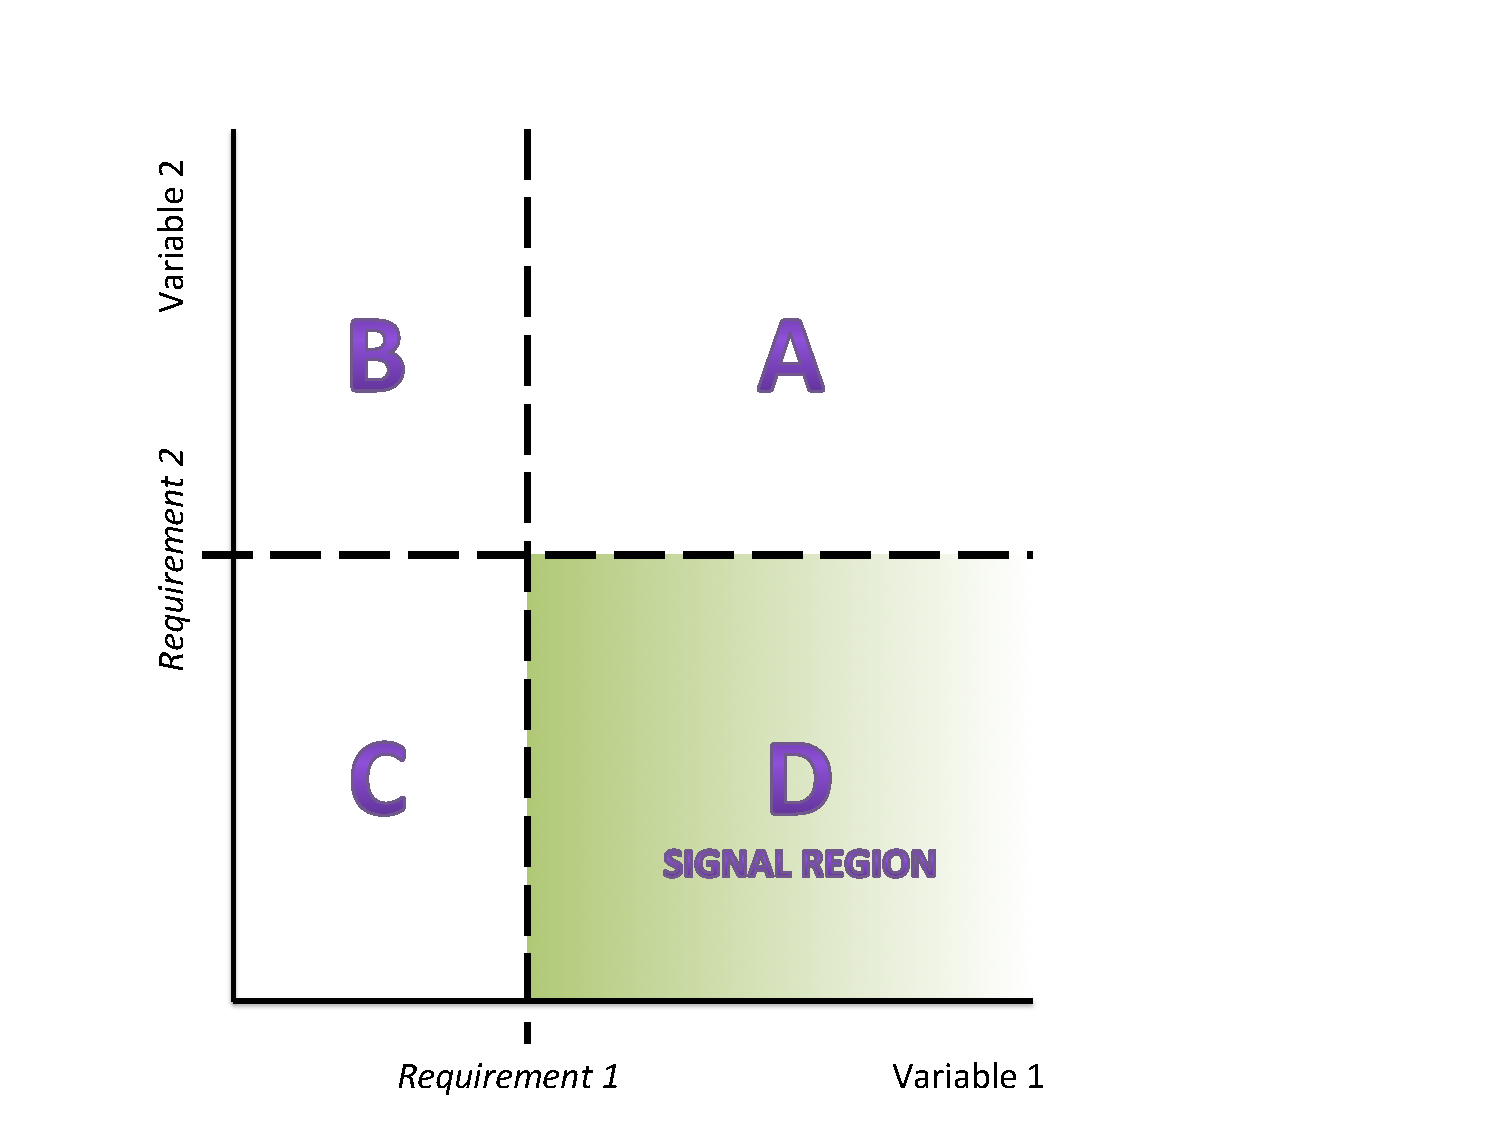
\includegraphics[width=0.6\textwidth]{images/Analysis/ABCD-req.pdf}
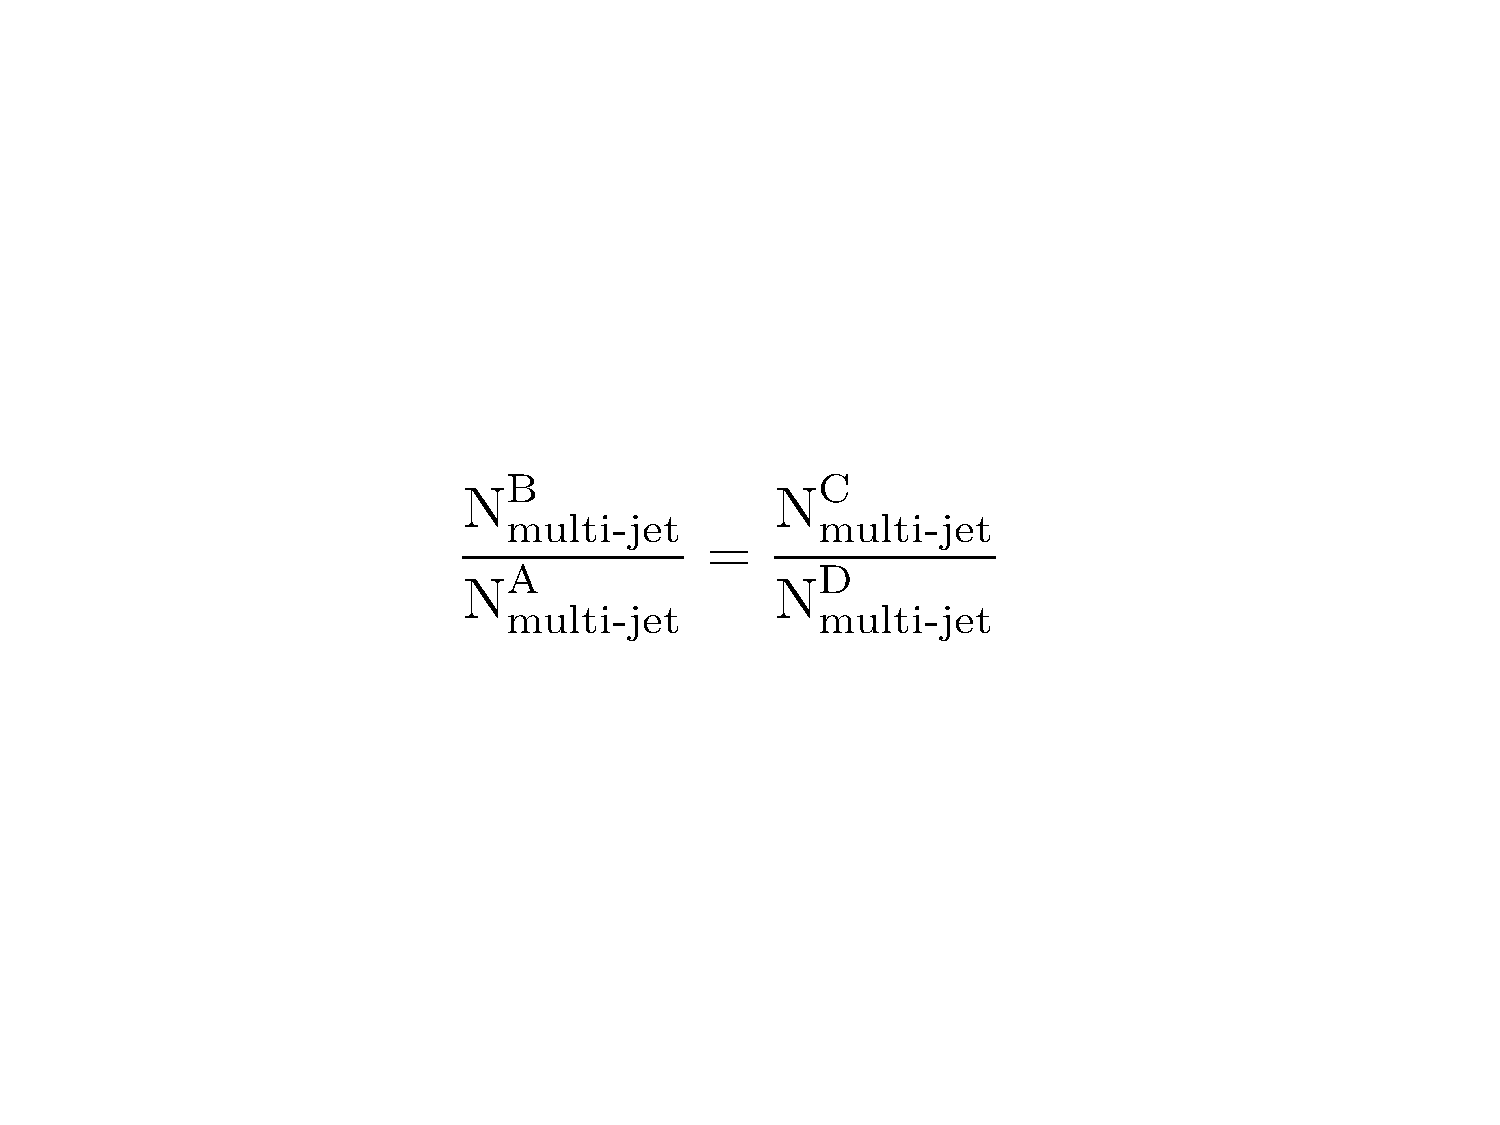
\includegraphics[width=0.6\textwidth]{images/Analysis/ABCD2.pdf}
}
\hspace{0.2cm}
\end{center}
\caption{Illustration of ABCD method}
\label{fig:ABCDdiagram}
\end{figure}

% \begin{equation}
% \frac{\textrm{N}^{\textrm{B}}_{\textrm{multi-jet}}}{\textrm{N}^{\textrm{A}}_{\textrm{multi-jet}}} = \frac{\textrm{N}^{\textrm{C}}_{\textrm{multi-jet}}}{\textrm{N}^{\textrm{D}}_{\textrm{multi-jet}}}
% \label{N-multi-jet}
% \end{equation}
For the background processes that are much more well modelled in simulation than QCD events, their yields in each region are subtracted from the data. This should in theory leave only QCD multijet events remaining and so the number of events in the signal region can be estimated from the equation in Fig.~\ref{fig:ABCDdiagram}. This method does have some dependence on the simulation and assumes that the other backgrounds are well modelled. The uncertainty on this assumption can be taken into account by varying the main \ttbar background by its main source of uncertainty. 


\section{Multi-variate analysis techniques ~\label{sec:MVAtechniques}}

Four top quark production events are very rare at the energies of $\sqrt{s} = $ 8~TeV and 13~TeV studied in this thesis. Typically, within the selection defined in Section~\ref{sec:Strategy} the main background is \ttbar production which is five orders of magnitude larger than the \tttt signal. In this type of analysis where the background and signal can be similar in many distributions and the signal is so rare, it can be advantageous to use multivariate analysis (MVA) methods to increase the signal to background separation. The main MVA method used in this thesis is \emph{Boosted Decision Trees} (BDT) where more details of this algorithm and its specific use in this analysis are given in the subsequent sections.


\subsection{Boosted Decision Trees}
\label{sec:BDT}

To start with, the simpler concept of a single Decision Tree will be considered. Decision trees are used to maximise the separation between a signal ($S$) sample and a background ($B$) sample by looking at a set of distributions in which there is some initial separation between the two; a training sample for each is provided to the algorithm. A simple decision tree is shown in Fig.~\ref{fig:DecisionTree} where each decision is defined at a \emph{node} and splits the dataset in two by placing a requirement in the most discriminating variable in order to separate as much background down one side and signal down the other side.
One can define the purity at each node as $P=\frac{S}{S+B}$. Another useful measure is the \emph{gain} at each node which gives a more symmetric measure of the node having high purity of either signal or background. The particular metric of gain used in this analysis is the commonly used \emph{Gini Index} which is defined as $Gini = P\cdot\left(1-P\right)$. A high Gini Index suggests the node contains a relatively equal amount of signal and background whereas a low Gini index shows that the node contains more of either signal or background. 
The goal is to scan across each distribution and find the requirement in the associated variable which maximises the \emph{separation gain} ($S_{G}$) as defined in equation~\ref{eqn:SepGain}. This process is iterated upon until a predefined end condition such as the maximum depth of the tree or the minimum number of events in a node.


% \begin{equation}
% P=\frac{S}{S+B}
% \label{eqn:Purity}
% \end{equation}

% \begin{equation}
% Gini = P\cdot\left(1-P\right)
% \label{eqn:Gini}
% \end{equation}

\begin{equation}
S_{G} = Gini(\textrm{parent}) - Gini(\textrm{child 1}) - Gini(\textrm{child 2})
\label{eqn:SepGain}
\end{equation}

\begin{figure}[h!]
\begin{center}
\subfloat{
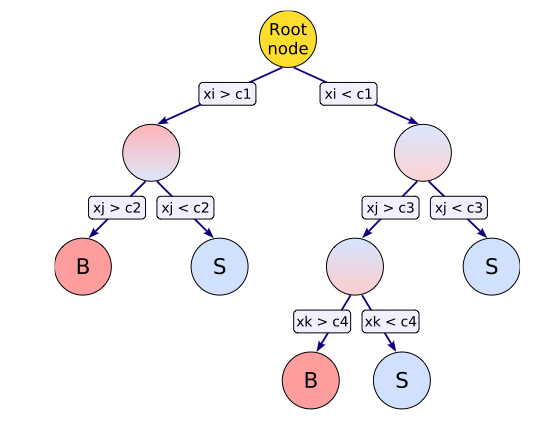
\includegraphics[width=0.67\textwidth]{images/Analysis/BDTFlow.png}}
\hspace{0.2cm}
\end{center}
\caption{Illustration of a single decision tree of depth = 3~\cite{2007physics3039H}.}
\label{fig:DecisionTree}
\end{figure} 

It has been found that using an ensemble (usually several hundred) of smaller decision trees of depth = 2 or depth = 3 is preferable to using one large decision tree as it can minimise \emph{overtraining}, ie. the propensity to train to the specific features of the training sample rather than the general trend. 

The first tree begins as a normal decision tree as described above and it terminates when it reaches the maximum depth defined. The error rate, $R_{err}$, of the tree is defined as the number of events incorrectly classified divided by the total number of events. The events which were incorrectly categorised are weighted according to equation~\ref{eqn:ErrorWeight} where $\alpha$ is the \emph{boost weight} which is dependent on $R_{err}$. The idea is that in the next iteration of a tree the incorrectly classified events are considered with higher importance. The degree of boosting can be adjusted by raising $\alpha$ to the power of $\beta$, the learning rate.

\begin{equation}
\alpha = \left( \frac{R_{err}}{R_{err}}  \right)
\label{eqn:ErrorWeight}
\end{equation}

This process is repeated until the predefined maximum number of trees has been reached. 

A discriminator value, $y_{BDT}$, is defined by summing the response from each tree, \emph{t}, and weighting each response by $\ln \left(\alpha_{t}\right)$ such that the trees with low error rates are considered more than trees with high error rates. The response from each individual tree is defined as $h\left(\textbf{x}\right)$ where $h\left(\textbf{x}\right) = +1 \textrm{ for signal and} -1 \textrm{ for background}$ and $\textbf{x}$ is the set of input variables. 

\begin{equation}
y_{BDT} = \frac{1}{Ntrees} \cdot \sum_{t}^{Ntrees} \ln \left(\alpha_{t}\right) \cdot h_{t}\left(\textbf{x}\right)
\end{equation}

Values of $y_{BDT}$ which are closer to +1 (-1) are considered to be more signal-like (background-like).

\subsection{Reconstruction of hadronic top quarks \label{sec:topreco}}

In \tttt single lepton channel there are three hadronically decaying top quarks while there is only one hadronically decaying top quark in the semi-leptonic \ttbar final state. Equivalently in the dilepton channel there are two (zero) hadronically decaying top quarks in \tttt (\ttbar). Therefore reconstructing top quarks from their hadronic decay products should be a powerful way to separate the signal and background processes. The jets which are in addition to the hard process in \ttbar are likely to come from initial or final state radiation (ISR or FSR) or from pileup, hence it should be unlikely to reconstruct a hadronic top quark from these additional jets. Due to the large number of jets within the selection, it is difficult challenge to find the right combination of jets which originated from a top quark. This motivates using multivariate analysis in order to rank each combination of three jets (tri-jet) according to which is most likely to be the combination that originated from a real hadronically decaying top quark.
A training sample from \ttbar events is provided to the BDT where the Monte Carlo truth information is used to classify whether a tri-jet combination was a \emph{good} combination which originated from a top quark or a \emph{bad} combination which is formed from random jets. The following variables were selected for use within the BDT:\\
\textbf{Tri-jet invariant mass} - Good tri-jet combinations should have an invariant mass distribution which peaks around the top mass.
Bad tri-jet combinations will have a much broader distribution. \\
\textbf{Di-jet invariant mass} - The di-jet combination is formed from the two jets with the smallest \DR separation. The invariant mass distribution should peak around the W mass for good tri-jet combinations.\\
\textbf{\ptrat} - This is the ratio of the vectorial \pt to the scalar sum of the \pt of the jets in the tri-jet combination. This is likely to be smaller in a random combination of jets where the vectorial \pt of each jet will cancel out more than in a good tri-jet combination.\\
\textbf{\DPTW} - This is the \Dphi between the tri-jet and di-jet system which should be smaller in good tri-jet combinations.\\
\textbf{\DPTb} - This is the \Dphi between the tri-jet and remaining jet not included in the di-jet system which should be smaller for good tri-jet combinations.\\
\textbf{\CSVj} - For the jet not used in the di-jet system, the CSV b-tagging discriminator value is used. If the di-jet system correctly identifies the quark jets coming from a W boson decay then the remaining jet in a good tri-jet combination should be a b-jet and hence will have a higher CSV b-tagging discriminator than a typical randomly selected jet.\\
The BDT algorithm is trained on the six variables above. It produces a discriminator value for each tri-jet combination. Higher BDT discriminator values are associated with the jets being more likely to have come from a top quark. Each tri-jet combination is ranked according to the BDT discriminator value. In the dilepton channel the value for the highest ranked tri-jet, known as BDT$_{tri-jet1}$, can be used as a discriminating variable between \tttt and \ttbar. In the single lepton channel the three jets which make up the highest ranked tri-jet combination are removed from the collection of jets and the process is repeated. The discriminator value of the next highest ranked tri-jet, BDT$_{tri-jet2}$, in this reduced jet collection can be used to distinguish between \tttt and \ttbar.

\subsubsection{Reduced Variables}
As mentioned above, BDT$_{tri-jet2}$ is calculated from a reduced jet collection where the three jets from the highest-ranked tri-jet are removed from the jet collection. In \ttbar events, the removal of the jets most likely to form a true top quark leave softer jets remaining in the reduced jet collection, usually from ISR, FSR or PU rather than the hard process of \ttbar production. In \tttt events the removal of the leading hadronic top quark candidate potentially leaves behind two additional hadronic top quarks, where some of the jets may not be reconstructed but there should still be harder jets from the hard process than what remains in \ttbar events. Therefore some discriminating variables can be formed from the reduced jet collection, as follows:

\textbf{HT$_{X}$} - This is the \HT of the reduced event which should be higher for signal \tttt events.\\
\textbf{\sumjetmassX} - Invariant mass of all jets contained in the reduced event which should be higher for signal \tttt events..

\subsection{Event-level BDT}

A second BDT is employed to increase the separation between the \ttbar background and \tttt signal beyond what can be achieved with a simpler variable. Several discriminating variables have already been formed from the hadronic top reconstruction; BDT$_{tri-jet1}$, BDT$_{tri-jet2}$, HT$_{X}$, \sumjetmassX. More discriminating variables can be formed from the event information, as follows:

\textbf{b-jet content}\\
As the branching ratio of top quarks to a b quark and a W boson is $\approx 100\%$, the main background process, \ttbar + \llbar,  typically produces two b-quarks while \tttt, typically produces four. Hence, the presence of more than two b-tagged jets is a potentially important source of discriminating power.
At 8~TeV this was exploited by looking at the number of CSVM b-tags in an event, \nMtags. At 13~TeV the CSV values for the \emph{third-highest CSV} and \emph{fourth-highest CSV} are used to discriminate between signal and background and it is expected that these values will be lower for \ttbar + \llbar events where the third-highest CSV and fourth-highest CSV are not likely to be b-jets. However for \ttbar + \bbbar events these variables do not provide much discrimination power.
Another variable used is the scalar sum of the \HT of all CSVM b-jets in the event which should be higher for \tttt events, \htb.

\textbf{Event-Activity}\\
One of the most obvious variables to choose to distinguish between \ttbar and \tttt is the number of jets (\njets) as on average \tttt events have a higher number of jets than \ttbar. In semi-leptonic \ttbar events there are up to four hard jets from the hard process compared to up to ten from \tttt, so the fifth and sixth jet \pt can be used to distinguish between the event types. The same idea is used to form the variable \htrat which is the ratio of the scalar sum of the \HT from the four highest \pt jets to the scalar sum of the \HT of the other jets in the events. This variable should be smaller for \tttt events where there are more than four jets coming form the hard process.
The \emph{centrality} of the event is defined as the ratio of the \HT in the event to the H in the event, where H is the scalar sum of the total momentum (P) in the event.

The lepton \pt is used as a training variable as it is slightly larger in \tttt events than in \ttbar events.

The \emph{Weighted jet multiplicity} (\njetsw) takes into account a combination of the \pt spectra of the jets and the differences in the jet multiplicity. It is sensitive to the differences between the \pt spectra of the jets from a top quark decay and those originating from ISR/FSR. The \njetsw definition is given in equation~\ref{eqn:WjetMul} where $p_T^{th}$ is the \pt threshold above which a jet is counted, $N_j\left(p_T > p_T^{th}\right)$ is the number of jets above the \pt threshold, $p_T^{low(up),i}$ takes values from the set [30 \GeV; $p_{T,1}$; $p_{T,2}\cdots$; $p_{T,N_j}$] ([$p_{T,1}$; $p_{T,2}\cdots$; $p_{T,N_j}$; 125 \GeV]), given that $p_{T,i}$ is the \pt of each jet in ascending order. The kinematic threshold is determined by the median jet \pt. The prefactor arises from the integral in the denominator combined with constant factors in the numerator.

\begin{equation}
% old version:	N_j^W = \frac{\int_{30}^{125}{N_j\left(p_T\mathrm{[GeV]} > p_T^{th}\right)\cdot p_T^{th}\,dp_T^{th}}} {\int_{30}^{125}{ p_T^{th}\,dp_T^{th}}} = \frac{1}{14725}\sum_{i=1}^{N_{jets}}{N_j\left(p_T\mathrm{[GeV]}>p_T^{low,i}\right)\cdot\left.\left(p_T^{th}\right)^2\right|^{p_T^{up,i}}_{p_T^{low,i}}},
N_j^W = \frac{\int_{30}^{125}{N_j\left(p_T > p_T^{th}\right)\cdot p_T^{th}\,dp_T^{th}}} {\int_{30}^{125}{ p_T^{th}\\
,dp_T^{th}}} = \frac{1}{14725}\sum_{i=1}^{N_{jets}}{N_j\left(p_T>p_T^{low,i}\right)\cdot\left.\left(p_T^{th}\right)^2\right|^{p_T^{up,i}}_{p_T^{low,i}}},  
\label{eqn:WjetMul}
\end{equation} 


\textbf{Training}\\
Each analysis from the single-lepton channel at 8~TeV, the single-lepton channel at 13~TeV and the dilepton channel at 13~TeV, uses different subsets of the variables described above. The variables which are only used in the dilepton channel have not been described here and can be found in \fxnote*{make appendix}{Appendix} The optimised set of variables for each training are provided to the TMVA package where the AdaBoost boosting algorithm is employed. The \tttt signal is trained against the main \ttbar background only as the other backgrounds are comparatively small. The \emph{event-level} BDT will return a discriminator value which will be closer to +1 (-1) for signal-like (background-like) events.

\section{Systematic uncertainties}
\label{sec:uncertainties}

Both the modelling of the simulation and the efficiency of the detector are not perfect and hence they bring some uncertainty to the measurement which needs to be taken into account when fitting the simulation to the data as described in section~\ref{sec:limitFit}.
There are two categories of systematic uncertainties; (i) Uncertainties which affect the normalisation of the distributions and (ii) uncertainties which affect the shape of the distributions. The quantity causing the uncertainty in each case can be varied up and down to produce alternative histogram templates.

\subsection{Normalisation uncertainties}
%The normalisation uncertainties will only affect the uncertainty on the expected limit rather than the limit itself when it is used in the template fit and limit setting procedure described in Section~\ref{sec:limit}.
Normalisation uncertainties include the following:
\begin{itemize}
\item \textbf{Luminosity}\\
There is some uncertainty on the luminosity as measured by the CMS Luminosity group which affects the normalisation of all simulation samples as they are scaled to the measured luminosity

% The CMS Luminosity Group give a recommendation of 2.6$\%$ uncertainty on the luminosity~\cite{CMS-PAS-LUM-12-001}.
\item \textbf{Monte Carlo simulation cross sections}\\
There is uncertainty on the cross sections given for each of the background processes due to uncertainty in the renormalisation and factorisation scale and the PDF uncertainty. As \ttbar is the main background to \tttt, the uncertainty on its MC cross-section is expected to be dominant over the other background processes. 

\item \textbf{Lepton ID, Iso and trigger SF}\\
An uncertainty arises from the choice of lepton triggers and identification criteria in the baseline selection which is applied to all simulation data sets.

%The uncertainty on \ttbar is ${}^{+2.5\%}_{-3.4\%} \left( \textrm{renormalisation and factorisation scale} \right)$ and ${}^{+2.5\%}_{-2.6\%} \left( \textrm{PDF} \right)$~\cite{PhysRevLett.110.252004}.
%\fxnote*{??}{The MC cross section uncertainties are modelled by assigning a $4\%$ uncertainty to each background process and a $10\%$ uncertainty to the signal process}
\end{itemize}

\subsection{Shape uncertainties}
 Shape uncertainties arise from the following quantities.
\begin{itemize}
\item \textbf{Factorisation and renormalisation scales}
This factorisation and renormalisation scale $\left(\mu_{f},\mu_{s}\right)$ can be shifted up and down at matrix element (ME) level and at parton shower (PS) level within the simulation. A shift in the $Q^{2}$ scale at PS level is equivalent to changing the value of $\alpha_{S}$ so the uncertainty from the jet multiplicity modelling in section~\ref{subsec:alphaS} can be included by inflating the PS scale systematic.

\item \textbf{Matching threshold}\\
The uncertainty due to the choice of matching threshold between the matrix element calculation and the parton shower is evaluated by producing alternative simulation samples where the matching threshold is varied between 20~GeV and 40~GeV.

\item \textbf{Generator choice}\\
The uncertainty on the choice of generator for the main \ttbar background is evaluated by considering an alternative \ttbar MC generator. The difference between the number of events in each bin of the output BDT distributions is converted into a symmetric uncertainty around the template created by the chosen MC generator.

\item \textbf{Jet Energy Scale}\\
The uncertainty on the \fxnote*{mentioned elsewhere?}{Jet Energy Corrections} applied to the simulation is evaluated by varying the Jet Energy Scale (JES) by $\pm 1\sigma$.

\item \textbf{JER}\\
The energies of the jets in simulation are smeared to match the observed discrepancy between the jet energy resolution, JER, in data and simulation. The amount the jet energies are smeared by is varied by $\pm 1\sigma$.

\item \textbf{b tagging}\\
There is a significant uncertainty on the measurement of b-tagging scale factors which is particularly important as variables derived from b-tagging jets are used in the event-level BDT. The method of accounting for this uncertainty varies depending on the b-tag modelling used from section~\ref{sec:btagModelling}.

\item \textbf{Pile up}\\
The minimum bias cross section used in the simulation which is used to derive the pile up scale factors is varied by $\pm 5\%$ to account for uncertainty on the minimum bias cross section. 

\item \textbf{\heavyflavourone~/~\heavyflavourtwo modelling}\\
The uncertainty on the measurement of the ratio of \heavyflavourone~/~\heavyflavourtwo is translated into an uncertainty on the scale factors applied to heavy flavour jets. An anti-correlated uncertainty is applied to light flavour jets.

\end{itemize}

The subsets of this list of uncertainties used for the \runone and \runtwo analyses and which data sets they are applied to are described in sections~\ref{c:Run1} and~\ref{c:Run2}. 

% The analysis procedure is repeated with \ttbar samples which have the respective quantity varied by $\pm 1 \sigma$ in order the produce new BDT templates with a deviated shape However, in the case of the matching threshold, the alternative shapes are produced by varying the matching threshold up to 40 GeV and down to 20 GeV.

\section{Limit setting \label{sec:limitFit}}
So far we have the nominal histogram templates in the BDT output discriminator disctribution for each background and signal, the normalisation systematic uncertainties for each source, and the alternative histograms for the up and down shape systematic uncertainties. All of these quantities are entered in the Higgs Combine Tool based on the Roostats package where a Maximum Likelihood Fit (MLF) is performed. In reality the MLF actually minimises the negative log likelihood ($-\ln\mathcal{L}$) as it is computationally simpler to work with.

The expected number of events in bin $i$, $\mu_{i}$, is given in equation~\ref{eqn:expectedmui} where L is the luminosity, $\sigma_{j}$ is the cross section for the source of events from process $j$, and $\epsilon_{ij}$ is the efficiency for source $j$ to be in bin $i$ derived from simulation

\begin{equation}
\mu_{i} = \sum_{j=1}^{n_{source}}L\sigma_{j}\epsilon_{ij}
\label{eqn:expectedmui}
\end{equation}

If we assume that the number of events in bin $i$, $n_{i}$, will be gaussian-distributed ($\mathcal{G}$) then the likelihood for the entire histogram is given in equation~\ref{eqn:gausslike}.
\begin{equation}
\mathcal{L} = \prod_{i=1}^{N} \mathcal{G}\left(n_{i}|\mu_{i},\sigma_{i}\right)
\label{eqn:gausslike}
\end{equation}

Each systematic uncertainty is modelled as a nuisance parameter in the fit. Normalisation uncertainties are modelled as lognormal nuisance parameters which is generally preferable to using a gaussian nuisance parameter as it is better at modelling multiplicative uncertainties and does not allow the parameter to become negative. The shape uncertainties are modelled using vertical morphing between the three templates; the nominal which has efficiency $\epsilon_{ij}^{0}$, systematic shifted up with efficiency $\epsilon_{ij}^{+}$ and systematic shifted down with efficiency $\epsilon_{ij}^{-}$. Quadratic interpolation is used between the two systematic templates and linear extrapolation beyond that range. The quadratic interpolation is shown in equation~\ref{eqn:VerticalMorphing} where morphing parameter $f$ has an Gaussian uncertainty with $\sigma_{f}=1$.

\begin{equation}
\epsilon_{ij} = \frac{f\left(f-1\right)}{2}\epsilon_{ij}^{-} - \left(f-1\right)\left(f+1\right) \epsilon_{ij}^{0}  \frac{f\left(f+1\right)}{2}\epsilon_{ij}^{+}
\label{eqn:VerticalMorphing}
\end{equation}

From the MLF, the number of background events from each source and the number of signal events can be extracted from the \emph{post-fit} distributions

\subsection{\CLS method}

The procedure used for setting limits on the strength of the signal process is the modified frequentist method known as the \emph{\CLS method}.
A test statistic, $\tilde{q}$, can be defined to distinguish between the background only (b-only) hypothesis and signal$+$background (s$+$b) hypothesis which includes the \tttt signal in the case of this analysis. The most common test statistic is the log likelihood ratio defined in eqn.~\ref{eqn:testStat}. The nominal signal strength, $\mu$, can be scaled by some factor and $\hat{\mu}$ is the parameter estimator of the signal strength. Equation~\ref{eqn:testStat} has the constraint of $0\geq \hat{\mu}\geq \mu$ to ensure that the signal strength is positive and to guarantee a one-sided confidence interval.

\begin{equation}
\tilde{q}_{\mu} = -2ln\frac{\mathcal{L}\left(data|s+b\right)}{\mathcal{L}\left(data|s\right)}
\label{eqn:testStat}
\end{equation}

% \begin{equation}
% \tilde{q}_{\mu} = -2ln\frac{\mathcal{L}\left(data|\mu,\hat{\theta}_{\mu}\right)}{\mathcal{L}\left(data|\hat{\mu},\hat{\theta}\right)}
% \label{eqn:testStat}
% \end{equation}

\begin{figure}[ht!]
\centering
    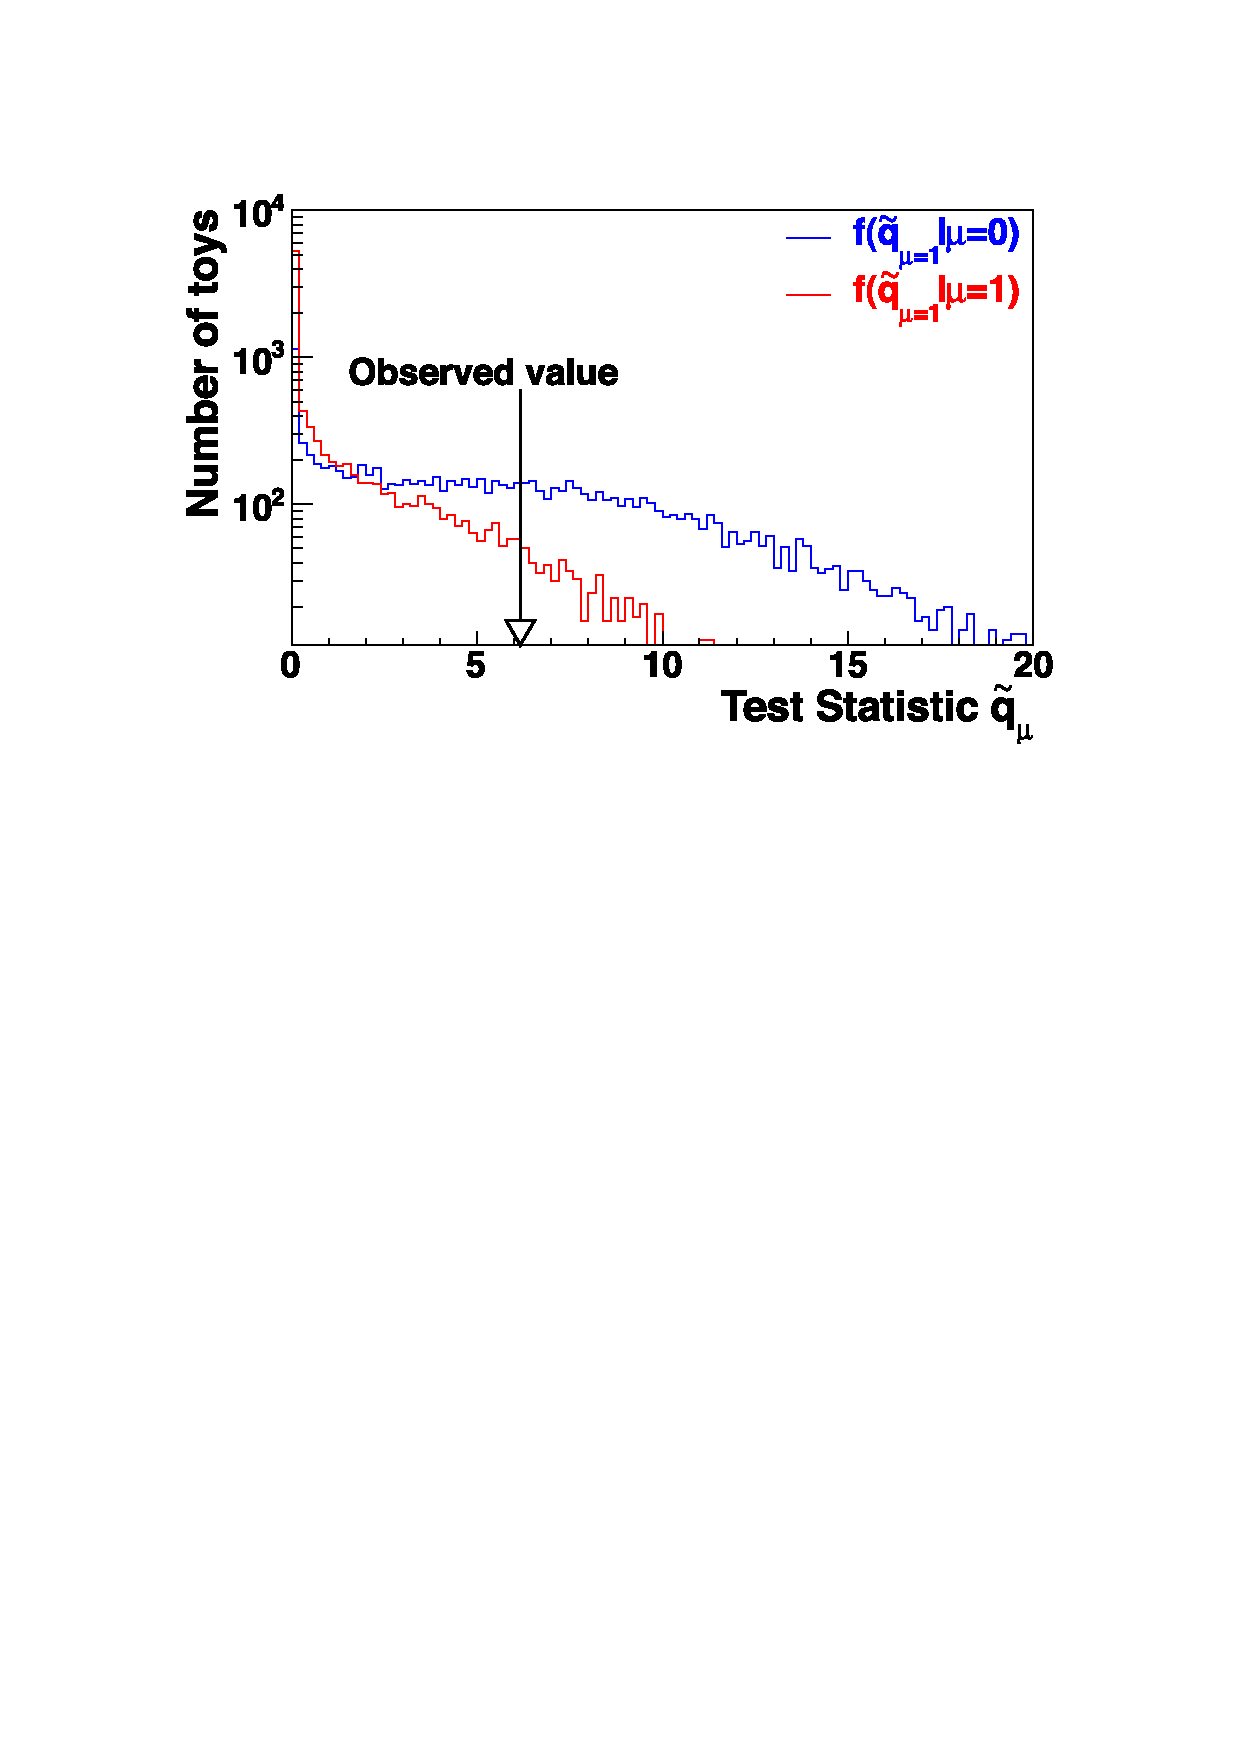
\includegraphics[width=0.5\textwidth]{images/Analysis/CLSdemo.pdf}
    \caption{Demonstration of the \CLS method~\cite{CMS-NOTE-2011-005}}
    \label{fig:CLSdemo}
\end{figure}

The value of $p_{s+b}$ denotes the probability of obtaining a value of $\tilde{q}_{\mu}$ which is equal or less likely to happen relative to the $q_{obs}$ given the s+b hypothesis.

\begin{equation}
p_{s+b} = \int_{\tilde{q}_{obs}}^{\infty} f\left(\tilde{q} | s+b   \right)_{\mu} d\tilde{q}_{\mu}
\end{equation}

One can similarly define $p_{b}$, however it is better to look at the definition of $1-p_{b}$ in equation~\ref{minuspb} as this is used in the \CLS definition in equation~\ref{eqn:CLS}.

\begin{equation}
1-p_{b} = \int_{q_{obs}}^{\infty} f\left(\tilde{q} |b   \right) d\tilde{q}_{\mu}
\label{eqn:minuspb}
\end{equation}


\begin{equation}
\CLS = \frac{p_{s+b}}{1-p_{b}} 
\label{eqn:CLS}
\end{equation}


We can say that our model is excluded with a $\left(1-\alpha \right)$ confidence level (C.L) if $\CLS < \alpha$ for a given signal strength, $\mu$. In this thesis 95\% Confidence Level upper limits are set on four top quark production within the standard model which corresponds to signal strengths which have $\CLS < 0.05$ being excluded.

% \begin{equation}
% p_{\mu} = \int_{\tilde{q}_{\mu}^{obs}}^{\infty} f\left(\tilde{q}_{\mu} | \mu, \theta^{obs}_{\mu}   \right) d\tilde{q}_{\mu}
% \end{equation}


% \begin{equation}
% 1-p_{b} = \int_{q_{0}^{obs}}^{\infty} f\left(\tilde{q}_{\mu} |0, \theta^{obs}_{0}   \right) d\tilde{q}_{\mu}
% \end{equation}
% \begin{equation}
% \CLS\left(\mu\right) = \frac{p_{\mu}}{1-p_{b}}
% \end{equation}

\subsection{Categorisation}
\label{sec:Cats}

Categorising events according to the numbers of jets and b-tags and hence producing more BDT templates to go into the fit allows the main \ttbar background to be constrained in the signal-depleted regions whereas the signal sensitivity will be increased in signal rich and background-depleted regions.


